\chapter{Implementation}

This chapter will include details on the implementation stage of the project. It will discuss the major sections of implementation, the tools used to carry out the implementation and any problems that were encountered whilst implementing the application.

\section{Overview}

The implementation stage of the project went very well, a few errors did arise but these were only ever minor errors and were quickly resolved. Using an IDE helped keep syntax errors to a minimum, which helped decrease the development time. The initial designs that were created, were followed and only 1 major change was made from the original designs. The majority of the time during this stage was spent implementing the data download services.

\section{IDEs that were used}

In this section I will discuss the two IDEs that were used whilst developing and the reasons why I switched from Eclipse to Android studio.

\subsection{Eclipse with Android developer tools}

When following the setup tutorials on the Android developer guide \cite{android_sdk}, the tutorial taught me how to install the Android developer tools (ADT) plugin for Eclipse \cite{eclipse}. I had already used Eclipse for other academic assignments so were already familiar with the basic user interface. 

The ADT plugin added the ability to create Android application’s to Eclipse. The plugin also provided a GUI interface for downloading Android SDK’s, including all documentation. The ADT plugin also allowed Eclipse to launch Emulators for a variety of devices.

As Eclipse is an IDE, when writing Android code with the ADT plugin installed code suggestions and syntax errors are shown in real time. Using an IDE greatly improved the speed at which I wrote code. As I was new to Android development the documentation suggestions provided whilst coding were extremely useful.

Eclipse is occasionally buggy when running on my computer, for example occasionally every line of code within the project will be highlighted as an error and I will therefore have to restart Eclipse for the error to disappear. Due to this error and a few other minor problems with Eclipse I searched the net for an alternative IDE half way through implementation.


\subsection{Android Studio}

Android Studio is an IDE created by the Android developers at Google \cite{android_studio}. Android Studio, which is currently still in beta is based off the IntelliJ IDEA IDE \cite{android_studio}. Although Android studio is still in beta \cite{android_studio}, the application works flawlessly, for everything that I needed it for.

As Android Studio was built solely for Android development it does not contain un-wanted  bloat like Eclipse. This makes it easier to find what you want in the menus as they contain fewer options. Android studio also has more intelligent code suggestions than Eclipses, making development easier. Android studio build configurations are configured using Gradle, which meant that adding library’s and custom build configurations was easy within Android Studio \cite{android_studio}.

After running into issues with Eclipse I found the early access preview of Android studio on Android developer website. Installing Android Studio was easy and the SDK’s and emulators I had downloaded within ADT were automatically transferred. Android Studio also provides an automatic migration manager to convert projects from Eclipse into Android Studio. I migrated the main application into Android studio, but never migrated the projects prototypes, as they were already complete at this stage in development.

\section{Use of Gradle}

Grade \cite{gradle} is an automatic build configuration tool, similar to Apache’s Maven. Gradle allows you create custom build configurations \cite{gradle} for a variety of setups. Gradle also has support for handling application dependencies, meaning importing and managing external libraries is easier and more efficient than manual methods.

I setup two build configurations using Gradle. The first configuration was used for building the application so that it was ready to be debugged. This configuration automatically enabled the debugable option within the Android manifest configuration file and also disabled Android’s ProGaurd \cite{progaurd}. Enabling the debugable variable allows the application to be ran in the Android Studio debugger and disabling ProGaurd prevented the built APK from being obfuscated and shrunk \cite{progaurd}, which improved the build time. 

The second build configuration that was setup was the configuration for building the release version of the application. This build setup disabled the debuggable options and enabled Android’s ProGaurd. Enabling ProGaurd prevents other developers from easily stealing your code as the generated code is obfuscated. Using ProGaurd also shrinks the file size and optimizes the final APK \cite{progaurd}.

On both of the above-mentioned build configurations I used Gradle to automatically check for the latest version of Robospice and download it if needed, including all of the needed dependencies. I found this feature extremely useful as Robospice had a list needed dependencies, that’d have to have been managed manually. 

\section{Test driven-development}

I had originally planned to follow the test-driven development pattern \cite{tdd} taken from the eXtreme programming \cite{xp} methodology throughout the project. As this was my first ever large project that I had used test-development I found using that it slowed down my development. As this project had a limit time scale, I decided to change the original plan of using test-driven development for the entire project to only using test driven development for critical classes such as the calculator and view drug activity. I then followed the waterfall model’s method of testing for the remaining classes, which is to test the application thoroughly once implementation was complete.

\section{Implementing the models}

The first package that I implemented for the project was the models package. The model’s had been first implemented within the prototypes, but the models had been slightly updated during the design stage, so these changes were made.

Implementing the models first allowed me to have classes to contain the data used for the system, meaning that classes that use the models will be able to use them.

\section{Database helper class}

Once the user models had been created, a database to store the models was implemented. The database helper class manages the database structure (creating and upgrading). The class also provides the rest of the classes with the ability to insert and retrieve data from the database. The implementation of this class went as expected and the class works excellently. Static variables were used throughout the class to allow the database to be customised easily.

\section{Authenticating the user}
The next part of the system to be implemented was the login activity and the authentication class. Implementing the authentication would allow the user’s username and password to be stored for the downloading of data, so this was logically the next step to implement.

When starting this project the only method of authenticating a user was to request a piece of data from the provided API and checking if an error was thrown, therefore I used the drug indexes API URL as this was the smallest XML file \cite{xml} to download. Although I used the smallest file possible whenever the login was successful the request would take several seconds as the drug index was downloaded. As the drug indexes were not used when logging in, this was a waste of data. To improve this I emailed the NHS representative and asked them to create an API URL.

The NHS \cite{nhs_website} implemented the newly requested API URL. This URL takes two parameters (the username and password of the user) and returns true or false if the credentials are correct. This new API URL greatly sped up the login process and improved efficiency.

\section{Downloading the data and populating the local database}

The next logical step was to implement the classes for downloading the database. Implementing the database and populating it early on ensured that all classes that used the data could be implemented afterwards. 

This is the section of the implementation stage that changed majorly from the initial design. In the original design I planned to carry out the task of downloading the data using AsyncTasks. As mentioned in the design chapter of this report, AsyncTasks were not appropriate for long running tasks \cite{async_task} as they’re attached to the activity. This meant that if the user minimised the application or changed the devices orientation the download would be cancelled. As the tasks of downloading all the data was not a short running task and that I wanted the user to be able to run the task in the background I could not use AsyncTasks.

As my original design would not work how I had expected I had to redesign the download classes. I then learnt about Robospice services \cite{robospice}, which would allow me to carry out the download in the background. Robospice services run in their own thread \cite{robospice} and therefore the download’s can be ran simultaneously through multi-threading.

Whilst using Robospice services I still encountered some problems. Robospice was not built for downloading data and storing it within the database, Robospice was built for long running HTTP requests \cite{robospice} such as downloading large images from the web. Due to the intended nature of the Robospice services the caching abilities of Robospice did not suit my application. This is because Robospice only caches the return value of the service, as my application adds the information to the database within the service, there is no return value. After researching into the best practices I learnt that Robospice has a class made specifically for tasks that are un-cacheable services \cite{robospice}, thus this class was extended in all of the applications services.

Another issue I encountered when implementing the download service was determining when all the services had finished downloading. If the user had the application open whilst the download was in progress the download task worked as expected as the on success and on failure methods of the activity were called, but if the user minimised the application and a service completed the task, when the service attempted to call the on success or on failure method nothing would occur as the activity would not exist at that point.

To solve this issue, extra methods had to be added to the DataProgress singleton, these extra methods keep track of the amount of started services and the number of completed services. To keep a track of the number of completed service I had to read into the Robospice service source code \cite{robospice} and plug into the method that notifies the activity when a service is complete, I then override this method and increased the finished count within the DataProgress singleton. When the number of started services is equal to the number of completed services then the all services have finished. The applications then checks that all the required API URLS have been downloaded, if they haven’t the user is notified of the failure and given the option to retry to download the parts that failed. 

The finished implementation of the download activity and service works excellently, both in the background and in the foreground. The user is notified of any errors, even if the errors occur in the background. If errors occur whilst in the background, when the user reopens the applications they are presented with the retry option. Whilst the download service is in progress a notification is placed into the notification centre, which allows the user to know the download is occurring.


\section{Main, browse and view drug activities}

Once the data download had been implemented it was possible to download the full set of data and store it within the applications local database. The next step was to display this data onto the screen. To achieve this the mock-up designs were implemented into the application for each of the views. Once user interface for each of the activities had been implemented the user interface was then populated using the data from the local database. 

The browse drugs page displays a list of all the drugs, which is taken from the drug indexes table. The user can enter text into the search box to filter the results within the list. Android ListAdapter provided an easy to use method for filtering the results automatically by just passing the filter text as a parameter to the filter method. 

Once the browsing of drugs had been implemented the next step was to implement the view drug page, a prototype of this page had already been made, so the prototype was copied into the project and edited to work with the new drug model. The implementation worked effortlessly and the drug data was displayed on the screen. 

There was a slight aesthetic issue with the displaying of data. The data provided from the API URL contained HTML. The native Android TextView object only has basic HTML support. The issue arose due to the references within the provided HTML using SUP tags. SUP tags in HTML are the tag used to super-script a piece of text, Android TextView HTML does support super scripts but the super scripts cause the line spacing to increase for lines that use super scripts. This made the drug’s information look misaligned which wasn’t aesthetically pleasing. 

To solve the aesthetic issues within the HTML I implemented a pre-parser to parse the HTML and replace all SUP tags with SMALL tags. Using SMALL tags made the references smaller, which made them standout, without affecting line height. I decided to execute the parsing during the displaying of the data rather than during the data download. Although this may not be the most efficient way of parsing the data, it ensures that the database contains an exact copy of original database.

As the prototype did not support the drug information header helpers this had to be implemented. An icon from the Glyphicon’s open source library \cite{glyph} was edited to match the colour scheme of the application. The icon was then added to the project and displaying of the icon where needed was implemented. To track which icon or header had been clicked Android’s tag feature was used, this allowed each header and icon to contain a tag of its ID within the database. When a clicks on the header the helper information corresponding to its tag is opened into an alert dialog.


\section{Calculator implementation}

The next classes to be implemented were the calculator classes.  I asked the NHS representative for information on the calculations and their equations during the first email I sent, they replied that they would be able to provide the information within the following week. This information had still not been received when the project had reached the stage in which the calculator would be implemented. Therefore I sent a further email to the representative asking for this information, as the representative was not in work at the time, they provided an excel spread sheet containing the data needed for the calculations and the C\# code that they used for the calculations. 

The C\# code was then read to derive the equations used for the calculations. Once the equations for calculation infusion rate from dosage and dosage from infusion rate were known the applications calculator and calculator activity class could be designed.

The data within the excel spread sheet was then converted into an XML file \cite{xml}, this XML file was then temporarily added to the project and the data parser for it was added to the data downloader. The NHS representative was then emailed, requesting them to implement an API URL for retrieving the data in the desired format. This allowed the development of the project to continue whilst the data was not accessible. The NHS representative later implemented the API URL and the calculator XML file was removed from the project.

As this class outputs information that could be lethal if incorrect a test-driven development \cite{tdd} approach was used whilst implementing it. As test data was needed, the NHS’s Medusa website \cite{medusa} was opened and a variety of calculations for multiple drugs were performed. The test data was then written into the unit tests, which would later be used to test the calculations.

The first method of the calculator to be implemented was the validation method. The purpose of this method is to return an integer value that represents the result of the validation. The possible integer values are stored as public static variables, meaning other classes can access their values, which is used when checking the result. The implementation began by creating test data that would return each of the available return types, such as success, invalid values and warnings. Once the test data had been written, the code to allow all the test cases to succeed was written. 

Once the validation method had been successfully implemented, the calculate method had to be implemented. As the test data for the calculator class had already been gathered the implementation to make the unit tests successful was the next step.

After every unit tests was successful the implementation of the calculator class was complete. The next class to be implemented was the calculator activity. The calculator activity class is responsible for providing the view to the user so that they can enter the information for the calculation. The design of the calculator activity allowed the user to select the type of calculation and the needed and un-needed fields were showing or hidden from the view. Hiding the un-need input fields helps improve the usability of the application. Once the user has entered the required information and clicked the calculate button, the information entered is validated. If the information passes validation the calculation is shown, otherwise the error is displayed using an Android Toast or a warning dialog is displayed if a warning is thrown \cite{dialog}. The design of the calculator activity was implemented successfully and activity works as expected.

\section{Showing the calculation performed}

It had been decided that the result of the calculation would be displayed within a dialog \cite{dialog}. The dialog had been designed so that the result of the calculation and the equations used to perform the calculation would be shown. The original plan was to display the equations within a TextView and use HTML to format the equations correctly.

It was decided that the HTML horizontal row (HR) tag would be used to display a horizontal line separating the numerator and denominator of the calculator equations. As Android TextView’s HTML support is limited, the HR tag is not available within TextView’s and therefore could not be used to display the calculation equations and results.

A WebView was used within then dialog to neatly present the user with the equation used and the results of the calculation. WebViews have larger HTML support than TextViews, they support both HTML and CSS. The calculation was displayed using HTML and then formatted using CSS. Relative font sizes were used within the WebView to ensure the result would be the same across devices. Once the WebView is displayed onto the screen the WebView is zoomed so that the HTML fills the dialog.

An extra benefit of using a WebView is that WebView’s allow the user to zoom in and out using a pinching motion with the fingers. This allows the user to make the equations and result smaller or larger should they want to.

The finished implementation successfully presents equations used and the result of the equations to the user. This allows the user to verify the correct calculation has been performed. 

\section{Adding access to the calculator}

Once the calculator classes had been created, a method of allowing the user to access the calculator was needed. To achieve this, the view drug activity was edited so that when a calculator is available for a drug, a button is displayed to open the calculator.

As only a limited number of drugs contain calculators I wanted to create a simple method for finding drugs that contain them. An activity similar to the browse drugs activity was created. This activity allows the user to search through a list of drugs that contains calculators. This activity speeds up the process of opening the calculator for the user.

\section{Extracting strings from the Java code}

Within Android you can define string variables within an XML file called strings.xml \cite{strings_xml}. By placing all strings used throughout the application within this file improves the maintainability and robustness of this system, as should future developers ever need to change the text contained within a string, they will only need to change the string within one file. Also using the strings.xml file allows future developers to easily provide extra language support\cite{strings_xml}.

Once the applications functionality was complete, code refactoring was executed to ensure that the code was efficient and easy to maintain. Whilst refactoring, all strings within the application’s code were extracted and placed into the strings.xml file \cite{strings_xml}. This will allow the NHS to quickly modify the text throughout the application, without needing to learn Android development. If the NHS would like to support the Welsh language within the application, which they may want to do, as the application was produced for NHS Wales, they only need to create a new directory for Welsh language support and then translate the strings.xml file into Welsh.

\section{Implementing XML customisability}
Early on in the projects lifecycle the NHS mentioned that they have multiple sets of data in a similar format to the data used for this application. They also mentioned that they plan to create multiple applications for the various data sets. The NHS asked for a simple method of modifying this application to allow them to create multiple applications from the other datasets. Throughout the design and implementation stages of the project this request was considered but not initially implemented, as it was additional extra, providing there was sufficient time.

As the implementation stage of the project ran as planned, there was enough time to implement the NHS’s request. To implement this functionality an addition xml file similar to the strings.xml \cite{strings_xml} file was created, called data\_download.xml. The purpose of the data\_download.xml file was to provide the API URLs at which the XML files containing the data could be requested. The data\_download.xml file also contains the XML tags that relate to database tables.

The API URLs provided within the data\_download.xml may contain two parameters, \%USERNAME\% and \%PASSWORD\%. The application will automatically replace these parameters with the users saved username and password. This allows the URLs to be changed by someone with very little programming experience.

To download the drug and drug information the application currently uses 26 URLs, one for each letter of the alphabet. Hard coding the URLS of the 26 sets of data would be bad software engineering. To accommodate for the multiple URLs, a list of the URLs and tags for them were added to the data\_download.xml file. The tags are used as a description of the URL that can be displayed to the used to relay feedback to the user, for example if an error occurred whilst downloading letters beginning with A, the application will alert the user by outputting “Failed to download letters beginning with A”, the tag in this case would be “letters beginning with A”. 

In order for the application to parse the data correctly, the XML tags \cite{xml} used within the data are described inside data\_download.xml. These descriptors include the tag name of the repeating element, for example the XML signifying the start of a new drug. The XML descriptors also include the tag names that contain the pieces of information that will be mapped to the database tables. By knowing the name of the repeating elements and the name of the tags containing the information within the repeating elements, the applications can populate the local database,

With both the customisability of the strings.xml file and the data\_download.xml file, a developer with no experience of Android development will be able to create multiple applications from varying API URL’s effortlessly. 


\section{Supporting older devices}
market
To improve the available reach of the application, it must support the earliest version of the Android SDK \cite{android_sdk} as possible. The minimum SDK required for the libraries and dependencies that were used was API version 8 \cite{robospice}. API version 8 (Froyo) was released on 20th May 2010 \cite{froyo}. The majority of Android users are currently on API version 8 or greater, it was therefore decided that the application must support all versions above API level 8 \cite{phone_market}.

During the implementation of the application a device running API version 19 was used. Once the implementation was complete, the minimum SDK version of the application was changed to API level 8 and ran on a device running Froyo \cite{froyo}. The application ran as it would on a newer device, only issues with the user interface were found.

When the application ran on the older device the custom colour scheme was not seen, this is because the customisation of the ActionBar was added at a later API version. Although the colour scheme was not seen, the application was still aesthetically pleasing.

On the older device the transparency of the buttons within the MainActivity was not applied, because of this the button was displayed, as a white button with white text thus the buttons text was not visible on the device. A new layout for the MainActivitiy, specifically for device earlier than API version 10 was created to fix the styling issue on the device. 

\begin{figure}[H]
  \centering
  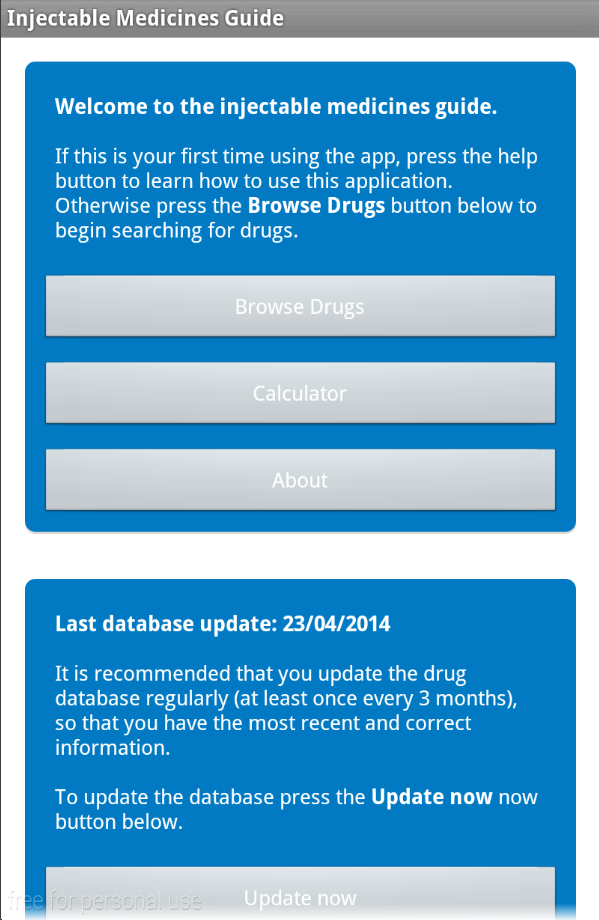
\includegraphics[width=11cm]{Images/screenshots/mainFailed.png}
  \captionof{figure}{Main activity on API 10 before improvement.}
\end{figure}

\section{Completed application screenshots}
This section includes screenshots of the final application, running on two devices, one running API version 10 and another running API version 18.  Android’s style changed greatly between these two versions, the screenshots prove that the application is aesthetically pleasing on both devices.

\begin{figure}[H]
\centering
\begin{minipage}{.5\textwidth}
  \centering
  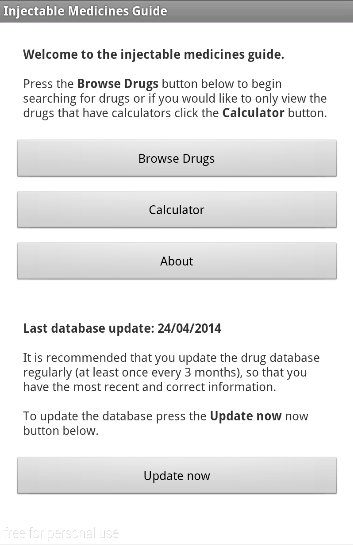
\includegraphics[width=.8\linewidth]{Images/screenshots/API10/main.png}
  \captionof{figure}{Main activity on API 10}
\end{minipage}%
\begin{minipage}{.5\textwidth}
  \centering
  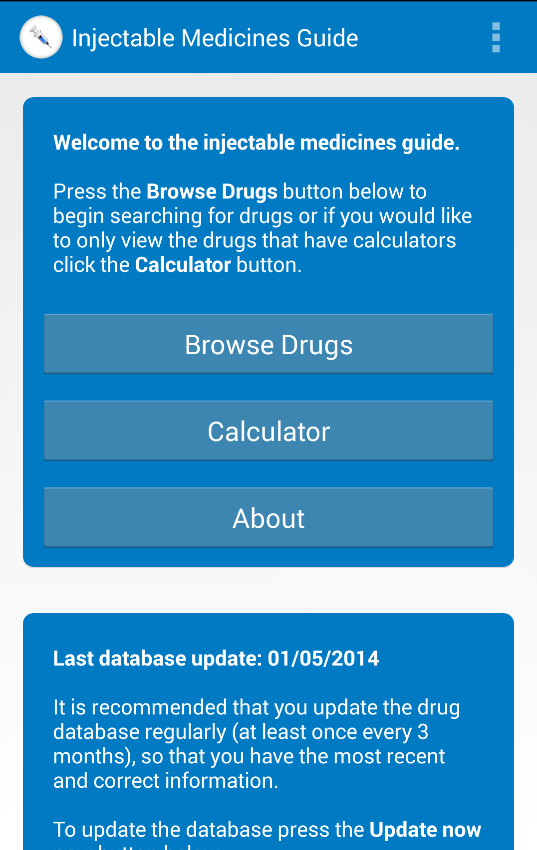
\includegraphics[width=.8\linewidth]{Images/screenshots/API18/main.png}
  \captionof{figure}{Main activity on API 18}
\end{minipage}
\end{figure}

\begin{figure}[H]
\centering
\begin{minipage}{.5\textwidth}
  \centering
  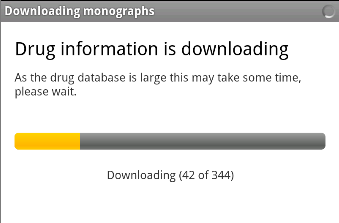
\includegraphics[width=.8\linewidth]{Images/screenshots/API10/download.png}
  \captionof{figure}{Download activity on API 10}
\end{minipage}%
\begin{minipage}{.5\textwidth}
  \centering
  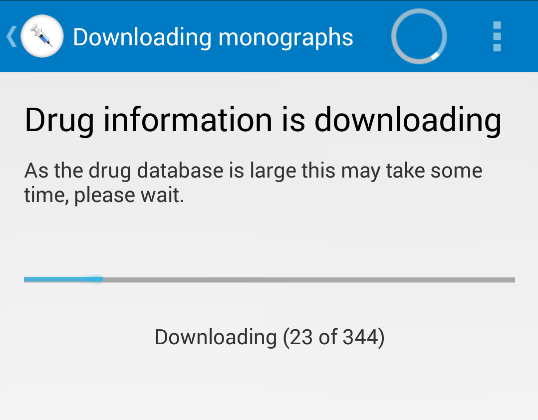
\includegraphics[width=.8\linewidth]{Images/screenshots/API18/download.png}
  \captionof{figure}{Download activity on API 18}
\end{minipage}
\end{figure}

\begin{figure}[H]
\centering
\begin{minipage}{.5\textwidth}
  \centering
  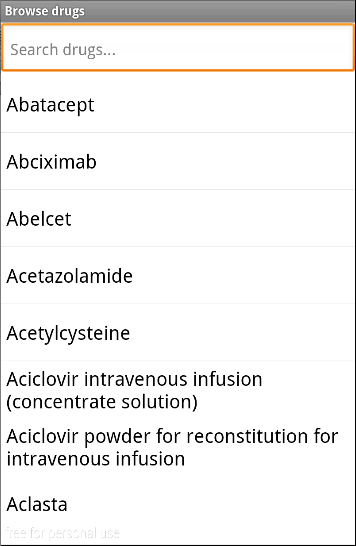
\includegraphics[width=.8\linewidth]{Images/screenshots/API10/browse.png}
  \captionof{figure}{Browse activity on API 10}
\end{minipage}%
\begin{minipage}{.5\textwidth}
  \centering
  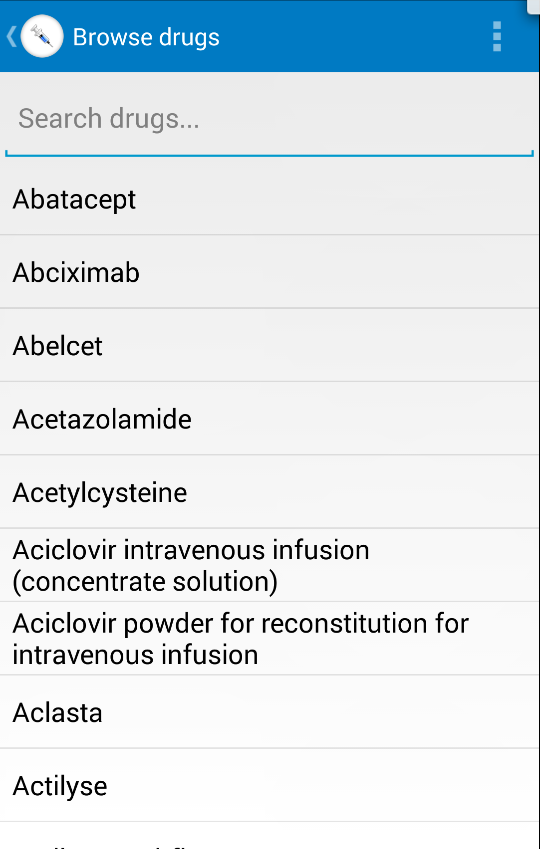
\includegraphics[width=.8\linewidth]{Images/screenshots/API18/browse.png}
  \captionof{figure}{Browse activity on API 18}
\end{minipage}
\end{figure}

\begin{figure}[H]
\centering
\begin{minipage}{.5\textwidth}
  \centering
  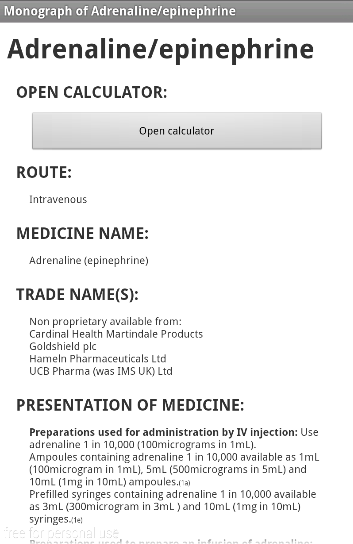
\includegraphics[width=.8\linewidth]{Images/screenshots/API10/view.png}
  \captionof{figure}{View activity on API 10}
\end{minipage}%
\begin{minipage}{.5\textwidth}
  \centering
  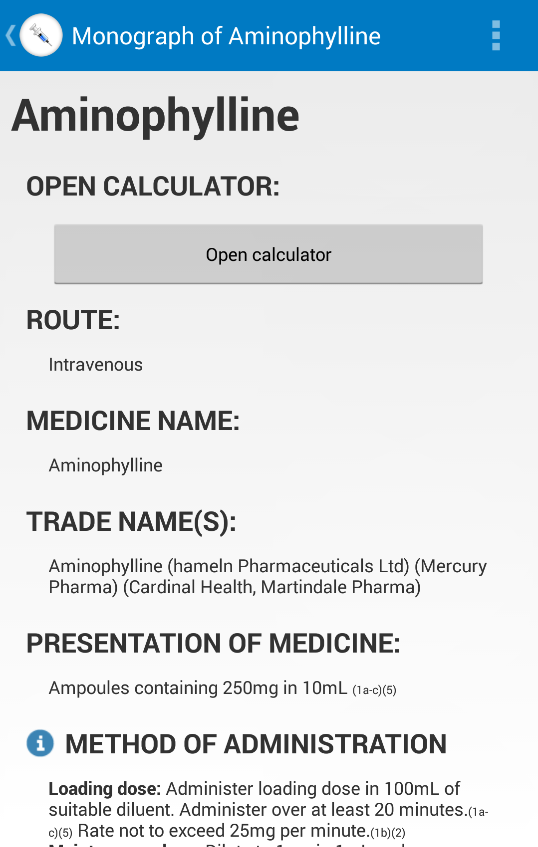
\includegraphics[width=.8\linewidth]{Images/screenshots/API18/view.png}
  \captionof{figure}{View drug activity on API 18}
\end{minipage}
\end{figure}

\begin{figure}[H]
\centering
\begin{minipage}{.5\textwidth}
  \centering
  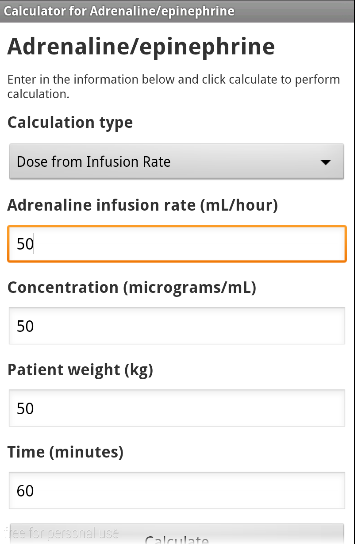
\includegraphics[width=.8\linewidth]{Images/screenshots/API10/calc.png}
  \captionof{figure}{Calculator activity on API 10}
\end{minipage}%
\begin{minipage}{.5\textwidth}
  \centering
  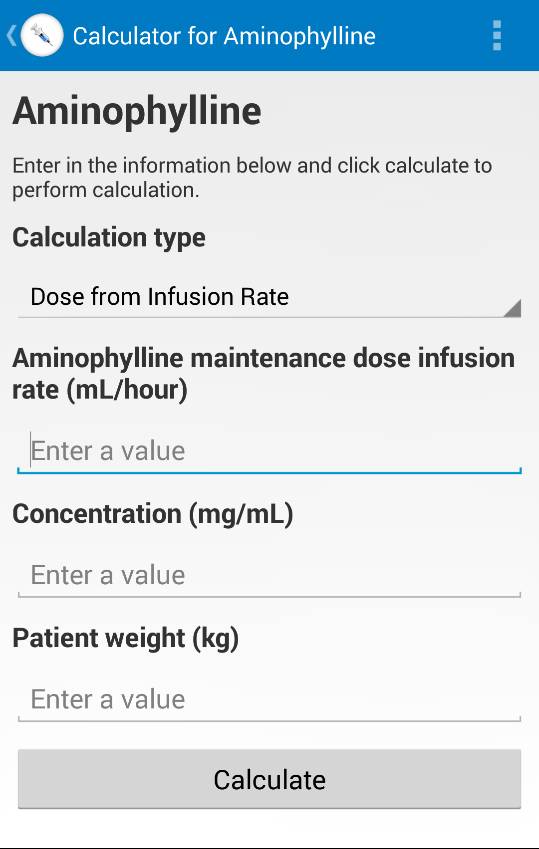
\includegraphics[width=.8\linewidth]{Images/screenshots/API18/calc.png}
  \captionof{figure}{Calculator activity on API 18}
\end{minipage}
\end{figure}

\begin{figure}[H]
\centering
\begin{minipage}{.5\textwidth}
  \centering
  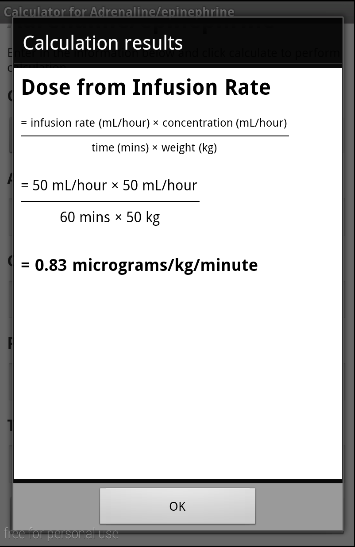
\includegraphics[width=.8\linewidth]{Images/screenshots/API10/calcResult.png}
  \captionof{figure}{Calculator result on API 10}
\end{minipage}%
\begin{minipage}{.5\textwidth}
  \centering
  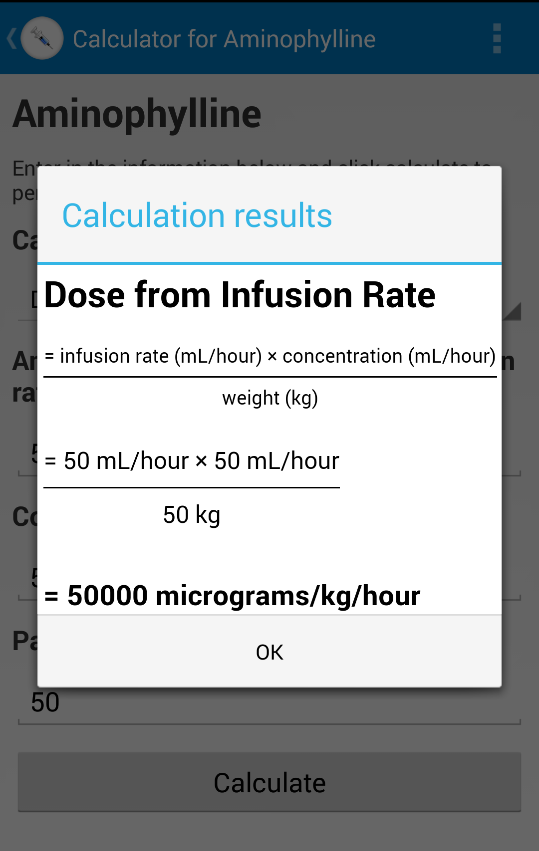
\includegraphics[width=.8\linewidth]{Images/screenshots/API18/calcResult.png}
  \captionof{figure}{Calculator result on API 18}
\end{minipage}
\end{figure}

